\chapter{Methods}
This chapters describes methods chosen for the project and the structures 

%What do I need methods for?

\section{Find meaning of Wikipedia Articles}
It is essential to know the meaning of the Wikipedia articles to be able to categorize them. 
%One of the most common ways
One way of finding the meaning of WIkipedia articles is by looking at Wikipedia's underlying structure since all Wikipedia articles are placed in categories. 

% One of the most commonly used strategies of finding the meaning of the articles is by looking at the 

\subsection{Representing the underlying structure}
Taking advantage of the underlying structure of Wikipedia requires a way of representing it. Each category has links to its subcategories, and links to the articles which are placed under the category (see figure \ref{fig:graphstructure}). Representing the structure could be split into two parts; representing the structure between categories, and representing the structure between categories and articles. 

\begin{figure}
\centering
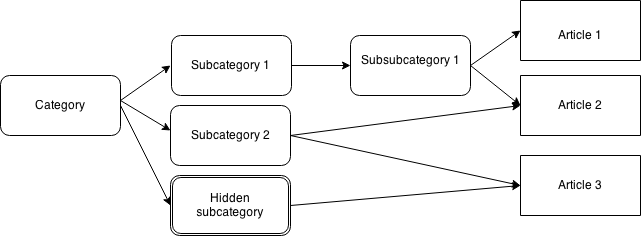
\includegraphics[width=\textwidth]{Chapters/Methods/graphstructure}
\caption{Simplified illustration of Wikipedia's category structure.}
\label{fig:graphstructure}
\end{figure}

\subsubsection{Category graph}
A category graph is a way of representing links between categories. This structure contains information about which categories can be reached from each category. Such a graph is represented with all subcategories of a category listed under the category. The results of this is a structure like the illustration in figure \ref{fig:categorystructure}).

%A category graph is a way of representing links between categories i.e., which categories can be reached from each category. The file containing all links between categories can be used to create such a graph. This is done by finding all subcategories of each category and remove all duplicate links. The results of this is a structure like the illustration in figure \ref{fig:categorystructure}).

\begin{figure}[h]
\centering
\begin{subfigure}[b]{0.4\textwidth}
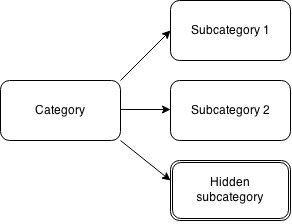
\includegraphics[width=\textwidth]{Chapters/Implementation/category-subcategories}
\caption{The structure where each category knows its subcategories}
\label{fig:categorystructure}
\end{subfigure}
\begin{subfigure}[b]{0.4\textwidth}
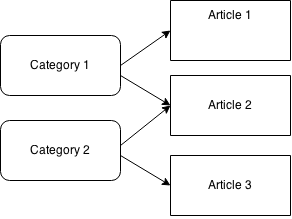
\includegraphics[width=\textwidth]{Chapters/Implementation/categories-articles}
\caption{The structure where each category know the title of its articles}
\label{fig:artstructure}
\end{subfigure}
\caption[The representation of the Wikipedia structure]{Combined this is the structure needed to represent the Wikipedia's underlying category structure as a graph}
\end{figure}

\subsubsection{Article graph}
A different structure is desirable for representing articles and their most describing categories (the categories shown at the bottom of the article page). The file containing all links between categories and their articles can be used to create a structure where each category knows its articles. Figure \ref{fig:artstructure}) illustrates this structure. 

%It is desirable to remove articles whose titles are not relevant for our project. Numbers without context is an example of Wikipedia article titles that are difficult to determine the meaning since a number could have various meanings, including temperatures, grades or years. Hence, all article titles which only contains numbers could be disregarded. Wikipedia contains many such articles, and a total of 23 227 articles where found. This reduces the number of links betweeen articles and categories as shown in table  \ref{tab:withoutnumber}.

\begin{comment}
It is important that the category names are equal all places they occur. Wikipedia is written by volunteers from all over the worlds, and users might use different encoding depending on where they are from. Thus, both a cleaning process and a normalization process should be performed on all category names. The cleaning process is to make the category names look readable, while the normalization is a process where all words are made equal regardless of character encoding \cite[p.~26]{iirbook}.

The cleaning process includes converting all words to lowercase, replacing underscores with spaces and splitting up all titles containing the code for newline (\emph{\textbackslash n}). Newline is a way of representing how the articles should be sorted, figure \ref{fig:withnewline} is an example of an \texttt{INSERT} statement with newline in the title of the category, where the category should be sorted as if the title was \emph{ducks} as seen in figure \ref{fig:fictionalbirds}. Hence, the relevant part of the category title is the part after the newline, and this is the part that is considered further in the results. 


\begin{equation}\label{eq:removehiddencat}
a = 0
\end{equation}
\end{comment}

\subsection{Representing category and article names}
\emph{Id mapping} is a storage efficient way of representing category names and article titles because category names and article titles usually are longer than their representing ids. The id mapper is implemented by creating a counter that assigns number to each category name or article title not already observed. 

\begin{comment}
The files containing the results becomes extremely large due to the size of the results. When writing all the results to file, the files becomes extremely large. All paths of all Wikipedia articles is more than 20 GB of compressed data. It is desirable to reduce the space needed for storing all results on the computer. The solution was to create an id mapping for each category name and article name. Id mapping gives all names a unique id, and instead of writing the full path of category names to the file, the full paths with category ids is written to file. 

The id mapping is implemented by creating a counter that assigns numbers to each category name or article name that is not found yet, i.e., a unique number represents each name. Figure \ref{fig:idmapping} shows an excerpt of the id mapping created for our purpose, where the id \emph{4600570} corresponds to the article about \emph{Ole-Johan Dahl}, which means that this id is used everywhere \emph{Ole-Johan Dahl} is used in paths. 

Id mapping is storage efficient because category names and article names usually are a  lot longer than their representing ids. 

Working with ids is also faster in many implementations concerning lookups in the program. This depends on the structure chosen for the programs, but when using dictionaries as done in our implementation, ids will perform faster than if using full names. An example of this can be seen in figure \ref{fig:id_lookup} where the time to find all categories from the category with id 177678 (corresponding to the category \emph{people}) is 0.955 minutes. Figure \ref{fig:fullname_lookup} shows the time needed to find the same paths for the category when using full names for categories and articles, which is found to be 1.559 minutes. Comparing the times shows that the time is a lot faster when using ids, which is important when many paths have to found.

The last reason to use ids instead of full names is that the full names may include characters useful for describing paths, for instance the characters "/" which is a common way of describing full paths. 

% Fordel 2: Kan bruke "/" in the text. 


\end{comment}

\section{Grading Categories}

% TODO: Find a good reference for this. 
Many Wikipedia articles can be reached from categories that are not describing for the content of the article. Thus, a grading has to be performed to find the most relevant paths for each article. 

\subsection{Grading based on Inlinks and Outlinks}
%\subsubsection{Inlinks and Outlinks of Categories}
Each category in Wikipedia has a set of parent categories i.e., categories that lead to the current category, and a set of subcategories i.e., categories that can be reached from the current category. The size of these sets for a given category can be notated as 
\begin{itemize}
\item \emph{Inlink} = number of parent categories
\item \emph{Outlink} = number of subcategories
\end{itemize}
Figure \ref{fig:Categorywparentandsub2} is a demonstration of how  inlink and outlink are connected to a category, and gives the idea that a catgory with high \emph{inlink} and \emph{outlink} are more likely to be visited when looking for paths for an article. 

\begin{figure}[h]
\centering
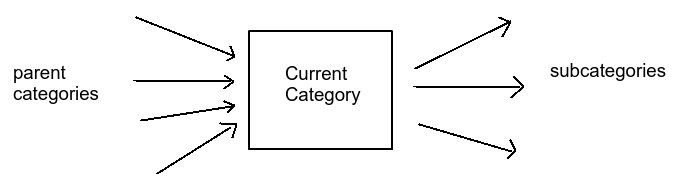
\includegraphics[width=\textwidth]{Chapters/Implementation/Grading/category_parent_sub}
\caption[Example of \emph{inlink} and \emph{outlink} for a category]{Example of how a category has links from parent categories and links to its subcategories. \emph{inlink} for the category is 4 and \emph{outlink} for the category is 3.}
\label{fig:Categorywparentandsub2}
\end{figure}

Two assumptions can be made from this. The first assumption is that categories with high inlink can be reached from categories that are not about the same. The other assumption is that categories with a high number for outlink are more likely to reach articles not necessarily connected to the category name since they can reach far in all the subcategories' directions. Thus, categories with a high value of outlink and a high value of inlink should have a lower score than categories seldom reached. 

\subsubsection{Scoring paths}
Grading based on inlinks and outlinks is done by finding the number of inlinks and outlinks for all categories in the structure, and the average number of inlinks and outlinks for all categories. Then the scoring should be weighted based on the values of inlink and outlink which leads to the following equation where $\xoverline{C_{in}}$ is the average \emph{inlink} and $\xoverline{C_{out}}$ is the average \emph{outlink}.  

%The assumption that categories with high \emph{inlink} and \emph{outlink} are more often visited leads to the thought that these categories should have a lower score than categories that are more rarly visited. 

%The first approach was therefore to find the \emph{inlink} and \emph{outlink} of all categories in the structure. These numbers had to be compared with the average number of \emph{inlink} and \emph{outlink} to know whether the number is high or low (see Table \ref{tab:avginlinkoutlink}). 


\begin{equation} \label{eq:categoryscore}
Score_{C} = \frac{inlink_{c} + outlink_{c}}{\xoverline{C_{in}} + \xoverline{C_{out}}}
\end{equation}

This means that the path score of a path $P$ is the sum of the scores of all categories (see equation \ref{eq:scoreinput}). 

\begin{equation} \label{eq:scoreinput}
Pathscore_{P} = \sum_{c} Score_{C}
\end{equation}

The problem with equation \ref{eq:scoreinput} is that short paths will be favored since there are fewer scores to be added together. A way of avoiding favoritism of short paths is by normalizing the path scores. 

\subsection{Normalized Grading based on Inlinks and Outlinks}
Grading based on inlink and outlink favors short paths even if the paths contains categories considered bad. One way of handling this problem is by normalizing the score of each path. Equation \ref{eq:normscoreinput} is a way of normalizing the path score of path $P$ so the length of the path does not determine the relevance of the path. 

% TODO: Write something about normalization - why is it good for grading?

\begin{equation} \label{eq:normscoreinput}
Pathscore_{P} = \frac{1}{N} \sum_{c} Score_{C}
\end{equation}
where $N$ is number of categories in the path.


\subsection{Deciding Relevant Paths}
One way of deciding which graded paths are relevant are by choosing a threshold for the path score. If the score is lower than a given score, it is marked as relevant and higher score means that it is not relevant. A threshold can be found by deciding how many paths 

The way to do this is to find the scores of all paths. and sort the scores from lowest to highest (see \ref{eq:sortedscores}). Then a $k$ has to be decided to how many paths are believed relevant of all paths, for instance one could assume that only 10\% of the paths are relevant, which leads to$ k = .10 \cdot n$. 

\begin{equation} \label{eq:sortedscores}
Sorted\_scores = \left[ S_{1}, S_{2}, ... , S_{k}, ... , S_{n} \right]
\end{equation}



\begin{equation} \label{eq:threshold}
T = Sorted\_scores[k]
\end{equation}


The problem with this method is that not all articles are guaranteed to have any relevant paths. The other problem is that the score of the path will vary a lot within different fields, since some of the Wikipedia articles are categorized under very specified categories. 
% TODO: Finn en kilde som er enig med meg. 

% Problem: 
% Finne hvor mange pather som er tilgjengelig. 

Another approach is to choose the best $k$ paths for each Wikipedia article. This approach is independent of the values on other articles' path score which means all Wikipedia articles are guaranteed at least one path. The disadvantage is that some paths might be marked as relevant even though their path score is lower than path scores marked as irrelevant by other articles. Another disadvantage is that articles with many good paths will still have to choose the best $k$ paths and good paths might be lost. 

\begin{comment}
Fordeler: ser ikke på de andre
alle articler får minst en score. 

Ulemper: mange gode - hvilken er best?
Kan ikke vite om scoren er god

\end{comment}


\section{Evaluation}
Evaluation the categorization is found by evaluating how well the classifier perform, in other words the correctness of the classifier.
%the correctness of the classifier
%The purpose of evaluating the classification is to determine  the correctness of the classifier 
%i.e., how well the classifier perform. 
This is done by finding the accuracy of the classifier, where the results from the classifier are compared with the correct results (called \emph{Gold Standard} \cite{wiki:goldstandard}). Equation \ref{eq:accuracy} \cite{wiki:accuracy} shows how the \emph{Rand Index (RI)} accuracy can be computed for the classifier. This equation measures the percentage of decisions that are correctcly classified by the classifier \cite[p:~330]{iirbook}.

\begin{equation} \label{eq:accuracy}
\text{acc}=\frac{\text{true positives}+\text{true negatives}}{\text{true positives}+\text{false positives} + \text{false negatives} + \text{true negatives}}
\end{equation}

\begin{table}[ht]
\centering
\renewcommand{\arraystretch}{1.25}
\begin{tabularx}{\textwidth}{l |X}
\textbf{Term}  & \textbf{Description} \\\hline
\textbf{True Postive} (TP) & Text is classified to the class by both classifier and \emph{Gold Standard}, (correct). \\ \hline
\textbf{True Negative} (TN) &  Text is neither classified to the class by the classifier, nor by \emph{Gold Standard}, (correct).  \\ \hline
\textbf{False Negative} (FN) & Text is not classified to the class by the classifier, but by \emph{Gold Standard}, (incorrect). \\ \hline
\textbf{False Positive} (FP) & Text is classified to the class by the classifier, but not by \emph{Gold Standard}, (incorrect).
\end{tabularx}
\\[10pt]
\caption{Explanation of the \emph{True Positive}, \emph{True Negative}, \emph{False Negative} and \emph{False Positive} \cite[p.~330-331]{iirbook}.}
\label{tab:}
\end{table}

Another way of evaluating the classifier is by using \emph{precision} and \emph{recall} which measures how many elements are correctly categorized and how many of the correct elements where found. 

%of evaluation categorization is with \emph{precision} and \emph{recall} which are measures of how many elements were correctly categorized \cite{wiki:precisionrecall}. P

Precision is defined as in equation \ref{eq:precision} \cite{wiki:precisionrecall}, which measure the fraction of returned results are relevant \cite[p.~5]{iirbook}. This means that precision can tell how many of the articles were correctly categorized. 

\begin{equation} \label{eq:precision} 
\begin{split}
\text{precision} & =\frac{|\{\text{relevant documents}\}\cap\{\text{retrieved documents}\}|}{|\{\text{retrieved documents}\}|} \\
 & = \frac{\text{TP}}{\text{TP} + \text{FP}}
 \end{split}
\end{equation}
Recall is a measure of finding how many of the relevant documents were found \cite[p.~5]{iirbook}. Equation \ref{eq:recall} \cite{wiki:precisionrecall} would provide information about how many of the correctly categorized elements where found. 

\begin{equation} \label{eq:recall} 
\begin{split}
\text{recall} & =\frac{|\{\text{relevant documents}\}\cap\{\text{retrieved documents}\}|}{|\{\text{relevant documents}\}|} \\
 & = \frac{\text{TP}}{\text{TP}+\text{FN}}
\end{split}
\end{equation}

Combining precision and recall gives a measure of the correctness of the classifier. And the measures can be combined to find the $F_{1}$-measure of the classifier which is way of measuring accuracy in terms of a weighted average of the precision and recall. The $F_{1}$-score is defined as in equation \ref{eq:fscore}\cite{wiki:fscore}. 

\begin{equation} \label{eq:fscore}
F_1 = 2 \cdot \frac{\mathrm{precision} \cdot \mathrm{recall}}{\mathrm{precision} + \mathrm{recall}}.
\end{equation}

The range of the $F_{1}$-score is between $0$ and $1$, where 1 is the best value. 

% TODO: vi kan også evaluaere mappingen mellom wikipedia articler og iab kategorier. 

%\subsection{Evaluate Wikipedia Categorization}
%\subsection{Evaluate Article Categorization}

\begin{comment}
Evaluation is the 


Kan også finne: 
p. 330 i iirbook. 
Rand index : measures the RI percentage of decisions that are correct. 
\end{comment}